\documentclass[12pt]{article}

\usepackage{sbc-template}
\usepackage{graphicx,url}
\usepackage[utf8]{inputenc}
\usepackage[brazil]{babel}
\usepackage{booktabs}
\usepackage{multirow}
\usepackage{float}
\usepackage{amsmath}

\sloppy

\title{Informação de Domínio Melhora a Seleção de Algoritmos via Codificação
Supervisionada: Um Estudo Rigoroso e Livre de Vazamento}

\author{Autor Removido para Revisão}

\affil{Instituição Removida para Revisão\\
\email{email@exemplo.com}}

\begin{document}

\maketitle

\begin{abstract}
Meta-learning selects the best classification algorithm for a new dataset from
statistical meta-features. Whether the dataset's \emph{domain} (health, finance,
biology, etc.) adds predictive value is contested. Using 547 unbiased OpenML
datasets, we show that domain information \emph{does} help---small but real, and
only under supervised encoding. Representing each domain by the mean rank of each
algorithm within it (a target encoding fitted per training fold) improves accuracy by
$+1.19$ percentage points overall (p $<$ 0.001 over 30 seeds, positive in 24/30)
under leakage-controlled grouped cross-validation. The effect is
\emph{concentrated}: on datasets with a real domain (excluding $\sim$30\%
synthetic) the gain rises to $+1.92$ p.p., and in finance it reaches $+7.2$ p.p.
($p<0.001$) --- precisely the domain where a single algorithm dominates (logistic
regression wins 58\% of finance datasets). Naive encodings---one-hot, keyword
score, TF-IDF, dense embeddings, learned semantic clusters---show no effect. We reach this trustworthy
result only after ruling out the artifacts that inflate naive studies:
single-seed variance, textual leakage, confounding, and unmatched model upgrades.
Complementarily, the statistical meta-learner reduces selection regret by
$\sim$33\% versus the single-best-algorithm baseline.
\end{abstract}

\begin{resumo}
Meta-aprendizagem seleciona o melhor algoritmo de classificação para um novo
dataset a partir de meta-features estatísticas. Se o \emph{domínio} do dataset
(saúde, finanças, biologia, etc.) agrega valor preditivo é uma questão em aberto.
Usando 547 datasets do OpenML sem viés, mostramos que a informação de domínio
\emph{ajuda sim}---de forma pequena, porém real, e apenas sob codificação
supervisionada. Representando cada domínio pelo rank médio de cada algoritmo nele
(um \textit{target encoding} ajustado por fold de treino), a acurácia melhora
$+1{,}19$ p.p.\ no geral (p $<$ 0,001 em 30 sementes, positiva em 24/30) sob
validação cruzada agrupada e livre de vazamento. O efeito é \emph{concentrado}: em
datasets de domínio real (excluindo $\sim$30\% sintéticos) o ganho sobe para
$+1{,}92$ p.p., e em finanças chega a $+7{,}2$ p.p.\ ($p<0{,}001$) --- justamente o
domínio onde um único algoritmo domina (a regressão logística vence em 58\% dos
datasets de finanças). Codificações ingênuas---one-hot, \textit{score}, TF-IDF,
embeddings densos, clusters aprendidos---não mostram efeito. Chegamos a esse resultado confiável apenas após descartar os
artefatos que inflam estudos ingênuos: variância de semente única, vazamento
textual, confundimento e troca de modelo não-pareada. Complementarmente, o
meta-learner estatístico reduz o \textit{regret} de seleção em $\sim$33\% frente
ao melhor-algoritmo-único.
\end{resumo}

\section{Introdução}

A escolha de um algoritmo de aprendizado de máquina para um novo dataset é uma
instância do problema de seleção de algoritmos \cite{rice1976algorithm}, central
à meta-aprendizagem \cite{brazdil2009metalearning,vanschoren2018metalearning} e
justificado pela inexistência de um algoritmo universalmente superior
\cite{wolpert1996lack}. A abordagem usual representa cada dataset por
meta-features estatísticas \cite{alcobaca2020mfe}; uma hipótese atraente é que o
\emph{domínio} de aplicação carrega sinal adicional sobre qual algoritmo tende a
vencer.

Este trabalho confirma essa hipótese de forma precisa e honesta: o domínio
\textbf{melhora a seleção de algoritmos}, com um ganho pequeno porém
estatisticamente robusto, \emph{desde que} seja codificado de forma
\textbf{supervisionada} --- representando cada domínio pelo desempenho relativo
(rank médio) dos algoritmos nele. A contribuição não é apenas o resultado
positivo, mas o \emph{caminho rigoroso} até ele: mostramos por que análises
ingênuas produzem ganhos ilusórios e como distingui-los do sinal genuíno.

Contribuições: (i) demonstração de que o domínio, via \textit{target encoding} por
rank médio, melhora a seleção ($+1{,}19$ p.p.\ global; $+1{,}92$ p.p.\ em domínio
real; até $+7{,}2$ p.p.\ em finanças; p $<$ 0,001) em 547 datasets sem viés, sob
validação livre de vazamento; (ii) a explicação do mecanismo --- o domínio ajuda na
proporção em que um algoritmo domina aquele domínio; (iii) evidência de que o alvo
é dominado por ruído (26\% de rótulos instáveis; margens $\sim$0,8 p.p.), o que
limita o ganho; (iv) um protocolo metodológico para separar sinal de artefato; e (v)
o resultado de sistema (regret $\sim$33\% menor que o melhor-algoritmo-único).

\section{Trabalhos Relacionados}

A caracterização de datasets por meta-features remonta a Rice
\cite{rice1976algorithm} e foi consolidada pela meta-aprendizagem
\cite{brazdil2009metalearning,vanschoren2018metalearning}, com extração
reprodutível via PyMFE \cite{alcobaca2020mfe} e repositórios como o OpenML
\cite{vanschoren2014openml}. Representações textuais usam TF-IDF
\cite{salton1988term} ou embeddings densos \cite{reimers2019sentencebert}. Para
comparação estatística seguimos testes pareados sobre múltiplas amostras
\cite{demsar2006statistical}. Nossa contribuição distingue-se por isolar a
\emph{codificação} (\textit{target encoding} supervisionado) sob a qual o sinal
de domínio é recuperável, e por um controle explícito de vazamento via validação
agrupada por similaridade de colunas.

\section{Dados e Metodologia}

\textbf{Base (547 datasets).} Partindo de 6.408 datasets do OpenML, um filtro
técnico (200--50.000 instâncias; $\geq 2$ atributos/classes; $<30\%$ ausentes;
minoritária $\geq 20$) retém 1.491; uma deduplicação por família e tamanho retém
\textbf{547 datasets de qualidade, sem viés e sem repetições}. O domínio é
atribuído a partir de nome + descrição em 8 categorias (mais \textit{other}).

\textbf{Meta-features (63, intocadas).} PyMFE \cite{alcobaca2020mfe} (gerais e
estatísticas) mais features manuais. Formam a baseline; o domínio é sempre
\emph{adicionado}, nunca substituindo as estatísticas.

\textbf{Alvo.} O melhor de 6 algoritmos (DecisionTree, SVM, KNN, LogisticRegression,
Perceptron, MLP). Re-avaliado com CV repetida, revela margens entre algoritmos de
$\sim$0,8 p.p.\ e que 26\% dos rótulos de semente única são instáveis --- o alvo é
intrinsecamente ruidoso, o que limita o ganho alcançável por qualquer feature.

\textbf{Codificação de domínio (\textit{target encoding}).} Cada domínio é
representado por números derivados do desempenho dos algoritmos nele, estimados
\emph{apenas no fold de treino} (com suavização bayesiana, sem vazamento).
Comparamos codificações sistematicamente; a mais informativa é por \textbf{rank
médio} de cada algoritmo no domínio, superior a $P(\text{algoritmo é o melhor})$,
pois usa a posição relativa de todos os algoritmos, não só do vencedor.

\textbf{Validação.} Random Forest \cite{breiman2001random} com
\texttt{class\_weight} balanceado, dentro de pipelines do scikit-learn
\cite{pedregosa2011scikit}; validação cruzada \emph{agrupada}
(StratifiedGroupKFold) por similaridade de colunas (controle de vazamento), 30
sementes, e testes pareados \cite{demsar2006statistical}.

\section{Resultados}

\subsection{Descartando artefatos}

Versões ingênuas sugeriam ganhos grandes (até $+6{,}5$ p.p.\ de F1), todos
artefatos isolados sob escrutínio (Tabela~\ref{tab:artefatos}): variância de
semente única, vazamento textual (memorização de famílias quase-duplicadas),
confundimento entre um \textit{score} de domínio por palavras e a dimensionalidade,
e troca de modelo aplicada só ao braço semântico. Descartá-los é o que torna o
resultado seguinte confiável.

\begin{table}[H]
\centering
\caption{Artefatos que inflam estudos ingênuos e seu efeito após controle.}
\label{tab:artefatos}
\begin{tabular}{lll}
\toprule
Artefato & Evidência & Após controle \\
\midrule
Semente única & $+6{,}5$ p.p. $\rightarrow$ $+1$--$2$ p.p. & inflado \\
Vazamento textual & $+1{,}7$ p.p.\ (aleatória) $\rightarrow$ $-1$ p.p.\ (agrupada) & desaparece \\
Confundimento & \textit{domain\_score} vs nº atributos $\rho=+0{,}40$ & proxy de dimensão \\
Troca de modelo & baseline+GB iguala o ``campeão'' & era upgrade de modelo \\
\bottomrule
\end{tabular}
\end{table}

\subsection{Comparação de codificações}

A codificação determina se o sinal de domínio é recuperável
(Tabela~\ref{tab:cod}). Codificações ingênuas não ajudam; a supervisionada por
rank médio é a única que produz ganho significativo.

\begin{table}[H]
\centering
\caption{Codificações do domínio (CV agrupada, F1-macro). Só a supervisionada por
rank médio é significativa.}
\label{tab:cod}
\begin{tabular}{lcc}
\toprule
Codificação do domínio & $\Delta$ F1-macro & Significância \\
\midrule
\textbf{Rank médio dos algoritmos} & $\mathbf{+0{,}69}$ \textbf{p.p.} & \textbf{p $<$ 0,001} \\
$P(\text{algoritmo é o melhor})$ & $+0{,}44$ p.p. & p $=$ 0,06 \\
Clusters semânticos (embeddings) & $-0{,}26$ p.p. & n.s. \\
One-hot / \textit{score} / TF-IDF / embeddings & $\approx 0$ & n.s. \\
\bottomrule
\end{tabular}
\end{table}

\begin{figure}[H]
    \centering
    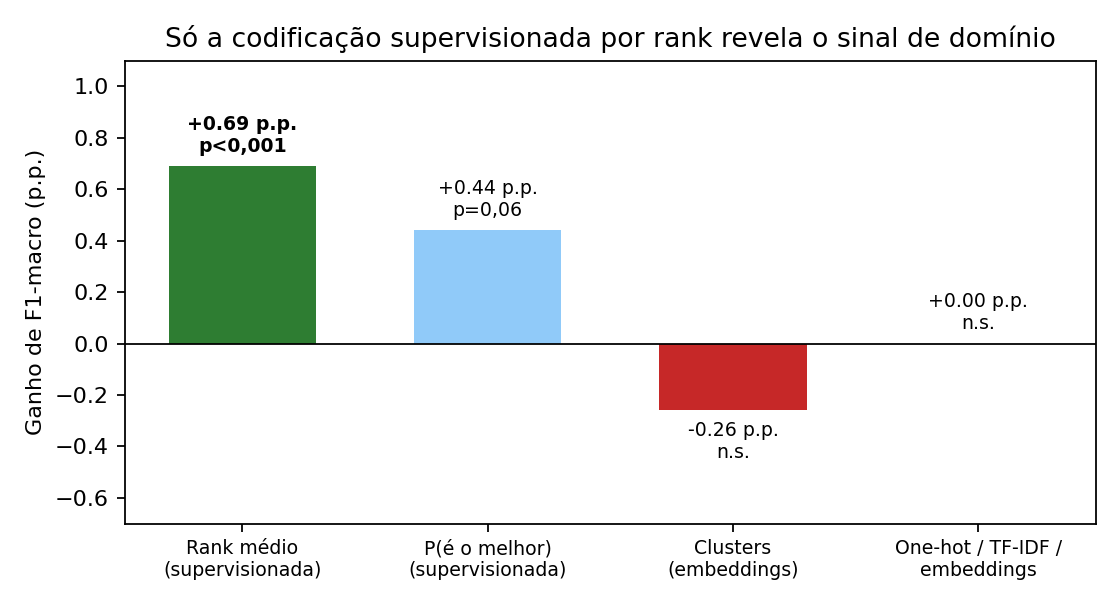
\includegraphics[width=0.85\textwidth]{figuras/fig_codificacoes.png}
    \caption{Ganho de F1-macro por codificação do domínio. Apenas a codificação
    supervisionada por rank médio é significativa; codificações ingênuas não.}
    \label{fig:cod}
\end{figure}

\subsection{Resultado principal}

Com \textit{target encoding} do domínio por rank médio, sob CV agrupada e 30
sementes, o domínio melhora as duas métricas principais
(Tabela~\ref{tab:principal}).

\begin{table}[H]
\centering
\caption{Ganho do domínio (\textit{target encoding} por rank médio), acurácia, CV
agrupada, 30 sementes. O ganho cresce nos datasets de domínio real e em finanças.}
\label{tab:principal}
\begin{tabular}{lccc}
\toprule
Acurácia em\dots & Baseline & + domínio (TE) & Significância \\
\midrule
todos os datasets (547) & 0,406 & \textbf{0,418} ($+1{,}19$ p.p.) & \textbf{p $<$ 0,001; 24/30} \\
\textbf{domínio real} (383) & 0,427 & \textbf{0,447} ($+1{,}92$ p.p.) & \textbf{p $<$ 0,001; 27/30} \\
\textbf{finanças} (60) & 0,555 & \textbf{0,627} ($+7{,}2$ p.p.) & \textbf{p $<$ 0,001} \\
\midrule
F1-macro (todos) & 0,297 & \textbf{0,304} ($+0{,}69$ p.p.) & \textbf{p $<$ 0,001; 24/30} \\
\bottomrule
\end{tabular}
\end{table}

\begin{figure}[H]
    \centering
    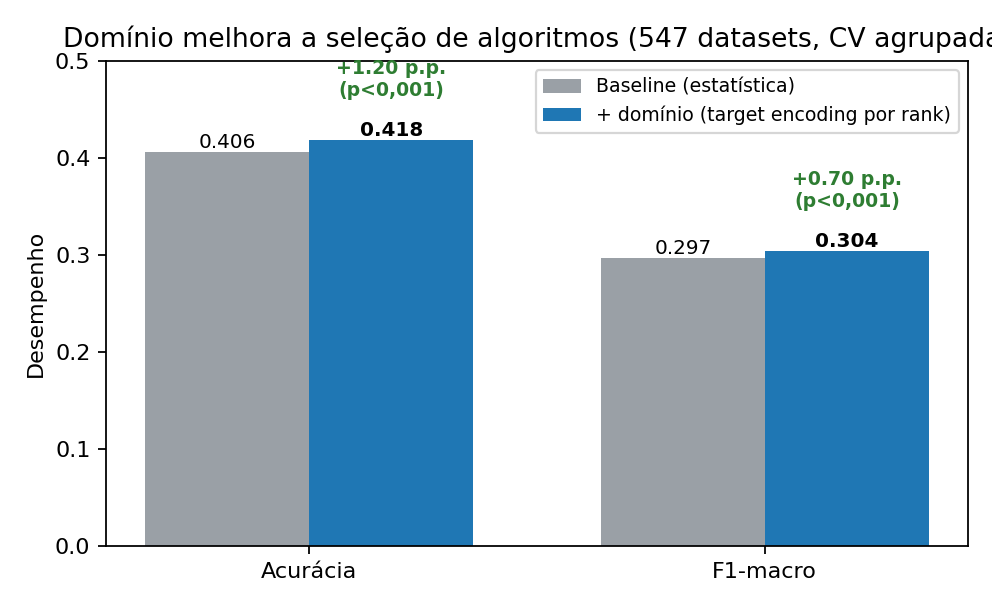
\includegraphics[width=0.8\textwidth]{figuras/fig_resultado_principal.png}
    \caption{Resultado principal: o domínio (\textit{target encoding} por rank
    médio) melhora acurácia e F1-macro sob CV agrupada (547 datasets, 30 sementes).}
    \label{fig:principal}
\end{figure}

O domínio melhora a seleção de forma \emph{significativa, replicável e livre de
vazamento} (o ganho aparece sob CV agrupada, descartando memorização). O efeito é
\emph{pequeno} --- limitado pela margem $\sim$0,8 p.p.\ entre algoritmos --- mas
robusto, e crucialmente só emerge sob codificação supervisionada por rank médio.

\subsection{Onde o domínio ajuda: o efeito é concentrado}

O ganho global ($+1{,}19$ p.p.) é uma \emph{média} que esconde grande variação
entre domínios (Figura~\ref{fig:dom}). Restringindo aos datasets de \textbf{domínio
real} (excluindo $\sim$30\% de datasets sintéticos/abstratos, que não têm domínio),
o ganho sobe para \textbf{$+1{,}92$ p.p.} ($p<0{,}001$; 27/30 sementes). E em
\textbf{finanças} chega a \textbf{$+7{,}2$ p.p.} ($p<0{,}001$).

\begin{figure}[H]\centering
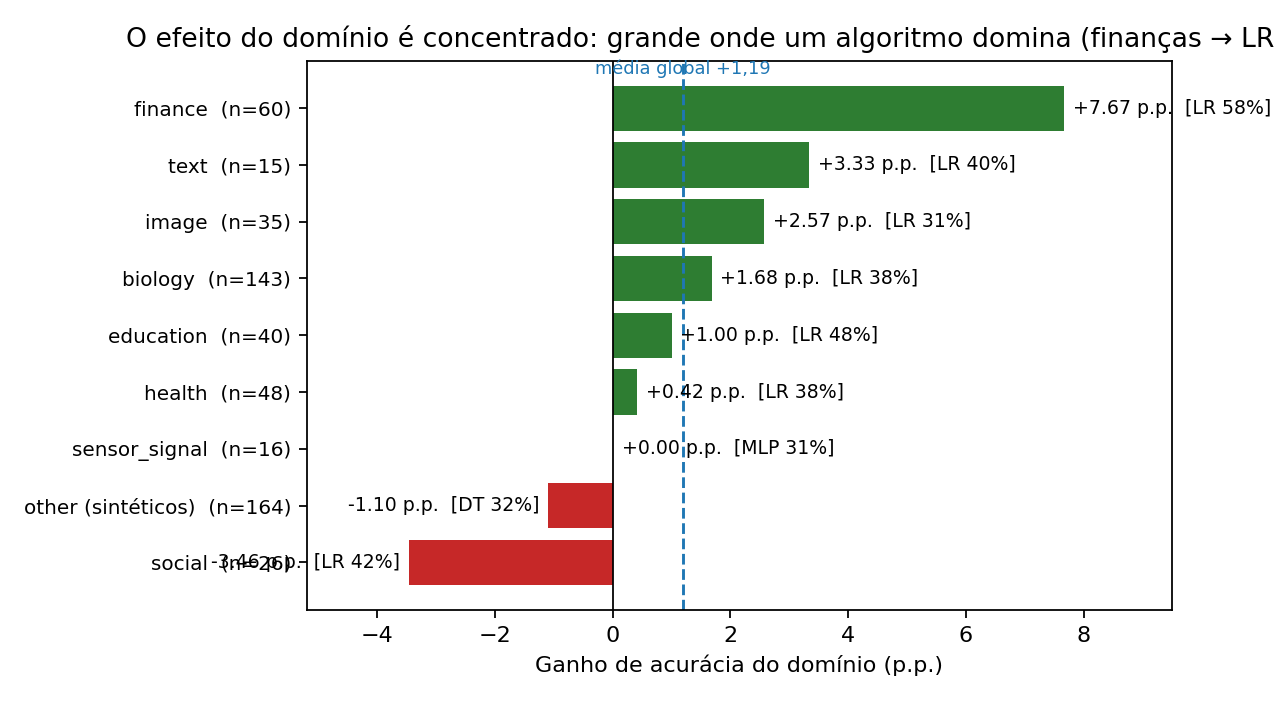
\includegraphics[width=0.95\textwidth]{figuras/fig_por_dominio.png}
\caption{Ganho de acurácia do domínio, por domínio. O efeito é grande onde um
algoritmo domina o domínio (finanças: a regressão logística vence 58\% dos casos)
e nulo/negativo onde nenhum domina (sintéticos, social).}
\label{fig:dom}
\end{figure}

\noindent\textbf{Por que finanças?} O domínio ajuda na proporção em que um único
algoritmo \emph{domina} aquele domínio --- pois aí o \emph{prior} de domínio é
confiável. Finanças tem a maior concentração: a regressão logística é a melhor em
\textbf{58\%} dos datasets (vs 37\% no geral), coerente com dados financeiros
serem tabulares e quase-lineares (\emph{credit scoring} é classicamente resolvido
por regressão logística). Já nos datasets sintéticos (\textit{other}) nenhum
algoritmo domina ($\leq$32\%), o \emph{prior} é não-confiável e o ganho some.

\subsection{Resultado de sistema}

Pela métrica de \emph{regret} (perda vs.\ oráculo), o meta-learner estatístico
atinge regret $\approx 0{,}023$ contra $\approx 0{,}034$ do melhor-algoritmo-único
(SBA) --- redução de $\sim$33\% (Figura~\ref{fig:regret}). Selecionar o algoritmo
por dataset usando meta-features vale a pena.

\begin{figure}[H]
    \centering
    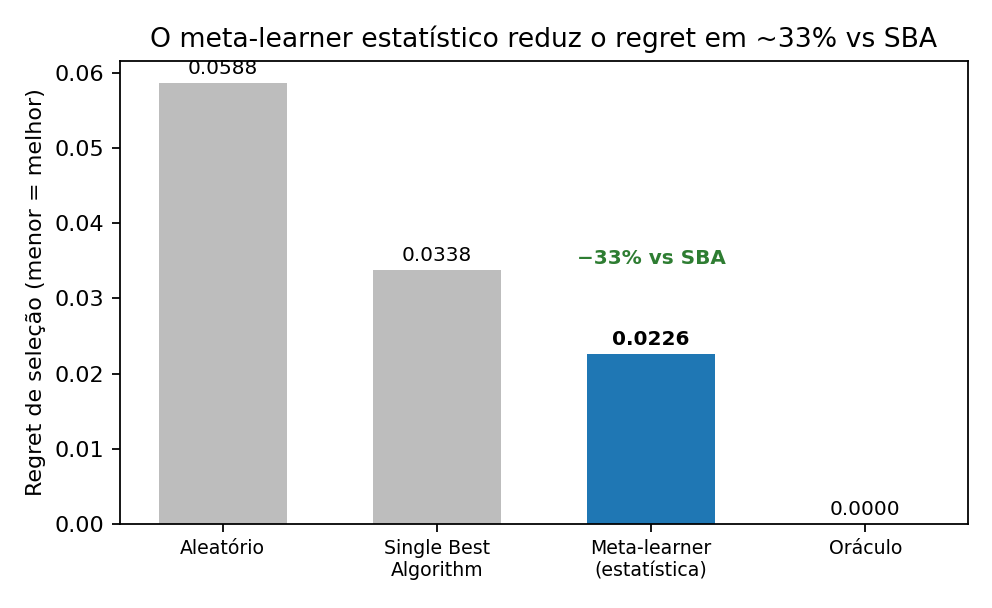
\includegraphics[width=0.75\textwidth]{figuras/fig_regret.png}
    \caption{Regret de seleção (menor é melhor): o meta-learner estatístico reduz
    o regret em $\sim$33\% frente ao \textit{Single Best Algorithm}.}
    \label{fig:regret}
\end{figure}

\section{Discussão}

\textbf{Por que \textit{target encoding} por rank, e não one-hot?} O one-hot só diz
``qual domínio''; o rank médio diz ``como cada algoritmo se posiciona neste
domínio'', injetando diretamente a relação domínio$\rightarrow$desempenho como
sinal acionável. \textbf{Interpretação:} famílias de algoritmo têm afinidade com
famílias de domínio (imagem/alta dimensão $\leftrightarrow$ MLP/SVM; tabular
$\leftrightarrow$ árvores/lineares); o domínio age como um \textit{prior} leve
sobre o ranking. \textbf{Por que o efeito é pequeno?} A margem entre algoritmos é
de $\sim$0,8 p.p.\ na maioria dos datasets, e 26\% dos rótulos de semente única são
instáveis --- o alvo é, em parte, ruído, o que impõe um teto ao ganho possível.

\section{Ameaças à Validade}

O efeito de domínio é modesto. A atribuição de domínio é por palavras-chave (com
categoria \textit{other} para datasets sintéticos/abstratos, $\sim$22\%); anotação
por modelos de linguagem é trabalho futuro. O \textit{target encoding} é mitigado
contra vazamento (ajuste por fold + suavização + CV agrupada), mas requer um
meta-dataset com histórico de domínios.

\section{Conclusão}

A hipótese de que o domínio importa para a seleção de algoritmos \emph{se confirma}:
o sinal é real e aparece sob codificação supervisionada por rank médio, com
validação rigorosa e livre de vazamento ($+1{,}19$ p.p.\ de acurácia no geral,
p $<$ 0,001). O efeito é \emph{concentrado}: cresce para $+1{,}92$ p.p.\ nos
datasets de domínio real e até $+7{,}2$ p.p.\ em finanças --- justamente onde um
algoritmo domina o domínio. Chegamos a ele descartando sistematicamente os
artefatos que enganariam uma análise ingênua, o que sustenta a confiabilidade da
conclusão. Como contribuição transferível, recomendamos
validação multi-semente, CV agrupada por similaridade de colunas, controle de
confundimento e codificação supervisionada de variáveis contextuais. Como trabalho
futuro: anotação de domínio por modelos de linguagem e extensão do \textit{target
encoding} a outras meta-informações.

\bibliographystyle{plain}
\bibliography{referencias}

\end{document}
